\documentclass{standalone}

\usepackage{tikz}
\usepackage{color}
\usepackage{helvet}
%\usepackage{gillius}
\usepackage{gitinfo2}
\usepackage{standalone}
\renewcommand{\familydefault}{\sfdefault}

\colorlet{redback}{red!85!black} 

\begin{document}

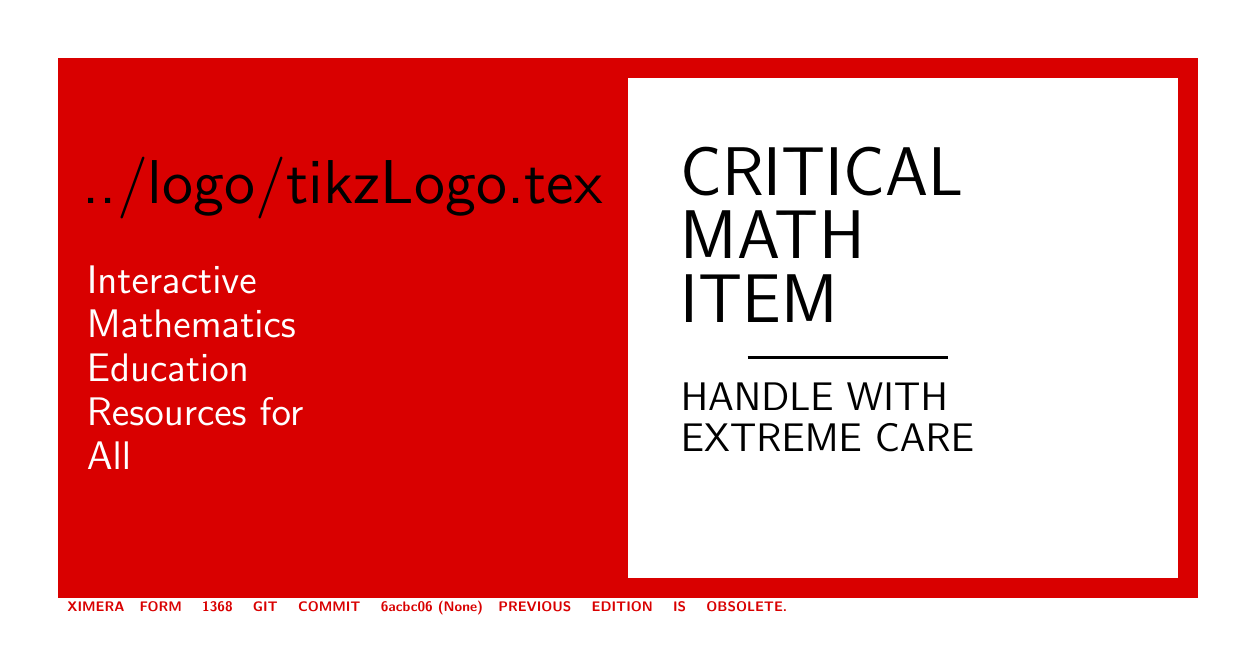
\begin{tikzpicture}[x=1in,y=1in] 
  \begin{scope}
    \clip(0,0) rectangle (6,3);
    \draw[fill=white,draw=none] (0,0) rectangle (6,3);
    \draw[fill=redback,draw=none] (0.15,.15) rectangle (5.85,2.85);
    \draw[fill=white,draw=none] (3,.25) rectangle (5.75,2.75);

    \node[anchor=west] at (.18,2.2) {\tikzset{draw/.append style={white}}
      \resizebox{2.6in}{!}{../logo/tikzLogo.tex}};
    \node[anchor=west,white] at (.247,1.3) [draw,align=left,draw=none]{
      \Large
      Interactive\\[.14cm]
      \Large
      Mathematics\\[.14cm]
      \Large
      Education\\[.14cm]
      \Large
      Resources for \\[.14cm]
      \Large
      All
    };
    
    \node[anchor=west,black] at (3.217,1.64)
         [draw,align=left,draw=none]{
      \Huge
      CRITICAL\\[.16cm]
      \Huge
      MATH\\[.16cm]
      \Huge
      ITEM\\[.7cm]
      \Large
      HANDLE WITH \\[.1cm]
      \Large
      EXTREME CARE
         };

    \draw[very thick,black] (3.6,1.35)--(4.6,1.35);          
    
    \node[anchor=west,redback] at (.15,.1) {\tiny\textbf{XIMERA\quad FORM \quad 1368 \quad GIT \quad COMMIT \quad 6acbc06 \gitAbbrevHash\quad PREVIOUS \quad EDITION \quad IS \quad OBSOLETE.}};
  \end{scope}
  \end{tikzpicture}
\end{document}
